
%(BEGIN_QUESTION)
% Copyright 2015, Tony R. Kuphaldt, released under the Creative Commons Attribution License (v 1.0)
% This means you may do almost anything with this work of mine, so long as you give me proper credit

\noindent
{\bf Lab Exercise -- introduction}

\vskip 5pt

Your task is to commission and de-commission a {\sl Wireless}HART field instrument, recording and/or controlling variables within that instrument using the Modbus protocol.  Each lab team will commission one {\sl Wireless}HART instrument (field device), and each person on that team will read or write one variable within that device.  Troubleshooting will be done on a PID-controlled process commissioned during a previous lab exercise, which may or may not be related at all to the {\sl Wireless}HART instrument you commission in this exercise.

The following table of objectives show what you and your team must complete within the scheduled time for this lab exercise.  Note how some of these objectives are individual, while others are for the team as a whole:

\underbar{Objective completion table:}

% No blank lines allowed between lines of an \halign structure!
% I use comments (%) instead, so that TeX doesn't choke.

$$\vbox{\offinterlineskip
\halign{\strut
\vrule \quad\hfil # \ \hfil & 
\vrule \quad\hfil # \ \hfil & 
\vrule \quad\hfil # \ \hfil & 
\vrule \quad\hfil # \ \hfil & 
\vrule \quad\hfil # \ \hfil & 
\vrule \quad\hfil # \ \hfil & 
\vrule \quad\hfil # \ \hfil \vrule \cr
\noalign{\hrule}
%
% First row
{\bf Performance objective} & {\bf Grading} & {\bf 1} & {\bf 2} & {\bf 3} & {\bf 4} & {\bf Team} \cr
%
\noalign{\hrule}
%
% Another row
Team meeting & mastery & -- & -- & -- & -- & \cr
%
\noalign{\hrule}
%
% Another row
Choose instrument and HART tag & mastery & -- -- & -- -- & -- -- & -- -- &  \cr
%
\noalign{\hrule}
%
% Another row
{\sl Wireless}HART instrument commissioned & mastery & -- -- & -- -- & -- -- & -- -- &  \cr
%
\noalign{\hrule}
%
% Another row
Choose instrument variable & mastery & & & & & -- -- -- -- \cr
%
\noalign{\hrule}
%
% Another row
Choose Modbus register(s) & mastery & & & & & -- -- -- -- \cr
%
\noalign{\hrule}
%
% Another row
Data displayed/controlled via Modbus & mastery &  &  &  &  & -- -- -- -- \cr
%
\noalign{\hrule}
%
% Another row
Circuit design challenge & mastery & & & & & -- -- -- -- \cr
%
\noalign{\hrule}
%
% Another row
Troubleshooting & mastery & & & & & -- -- -- -- \cr
%
\noalign{\hrule}
%
% Another row
Lab question: {\sl Wireless}HART theory & proportional &  &  &  &  & -- -- -- -- \cr
%
\noalign{\hrule}
%
% Another row
Lab question: Commissioning & proportional &  &  &  &  & -- -- -- -- \cr
%
\noalign{\hrule}
%
% Another row
Lab question: Mental math & proportional &  &  &  &  & -- -- -- -- \cr
%
\noalign{\hrule}
%
% Another row
Lab question: Diagnostics & proportional &  &  &  &  & -- -- -- -- \cr
%
\noalign{\hrule}
%
% Another row
Decommission and lab clean-up & mastery & -- -- & -- -- & -- -- & -- -- &  \cr
%
\noalign{\hrule}
} % End of \halign 
}$$ % End of \vbox

The only ``proportional'' scoring in this activity are the lab questions, which are answered by each student individually.  A listing of potential lab questions are shown at the end of this worksheet question.  The lab questions are intended to guide your labwork as much as they are intended to measure your comprehension, and as such the instructor may ask these questions of your team day by day, rather than all at once (on a single day).

\vskip 10pt

{\bf It is essential that your team plans ahead what to accomplish each day.  A short (10 minute) team meeting at the beginning of each lab session is a good way to do this, reviewing what's already been done, what's left to do, and what assessments you should be ready for.  There is a lot of work involved with building, documenting, and troubleshooting these working instrument systems!}

As you and your team work on this system, you will invariably encounter problems.  You should always attempt to solve these problems as a team before requesting instructor assistance.  If you still require instructor assistance, write your team's color on the lab whiteboard with a brief description of what you need help on.  The instructor will meet with each team in order they appear on the whiteboard to address these problems.






\vfil \eject

\noindent
{\bf Lab Exercise -- team meeting}

\vskip 5pt

An important first step in completing this lab exercise is to {\bf meet with your instructor} as a team to discuss safety concerns, team performance, and specific roles for team members.  If you would like to emphasize exposure to certain equipment (e.g. use a particular type of control system, certain power tools), techniques (e.g. fabrication), or tasks to improve your skill set, this is the time to make requests of your team so that your learning during this project will be maximized.

For example, if a team member lacks experience using personal computers, this lab exercise is an excellent opportunity to gain those skills.  It is {\it strongly} recommended that those team members with the least computer experience be the people to do all the initial configuration work while those with more experience merely supervise.

Remember, the purpose of this lab exercise is not to complete it in the least amount of time, but rather for every team member to gain new knowledge and skill.  This is why tasks should not necessarily be assigned with {\it maximum efficiency} in mind as they would at a workplace, but rather with {\it maximum learning} in mind because this is a school.

\vskip 30pt









\vfil \eject

\noindent
{\bf Lab Exercise -- circuit design challenge}

\vskip 5pt

Connect a loop-powered ``smart'' differential pressure transmitter (4-20 mA output with HART communication ability) to a DC voltage source and a meter such that the meter will indicate a increasing signal when a certain stimulus is applied to the transmitter, setting the transmitter's pressure measurement range as specified by the instructor.  All electrical connections must be made using a terminal strip (no twisted wires, crimp splices, wire nuts, spring clips, or ``alligator'' clips permitted).  You are expected to supply your own tools and multimeter.

This exercise tests your ability to navigate a ``smart'' instrument's parameters using a communicator as well as properly interpret terminal connections on a field instrument for signal and power.

$$\includegraphics[width=15.5cm]{i03627x01.eps}$$

\vskip 10pt

The following components and materials will be available to you: assorted 2-wire 4-20 mA differential pressure {\bf transmitters} calibrated to ranges 0-30 PSI or less, equipped with Swagelok compression tube connectors at the ``high'' and ``low'' ports ; lengths of {\bf plastic tube} with ferrules pre-swaged ; {\bf terminal strips} ; lengths of {\bf hook-up wire} ; 250 $\Omega$ (or approximate) {\bf resistors} ; analog {\bf meters} ; {\bf battery clips} (holders); {\bf HART communicator}.

\vskip 10pt

\noindent
{\bf Transmitter range} (instructor chooses): \hskip 20pt LRV = \underbar{\hskip 50pt} \hskip 20pt URV = \underbar{\hskip 50pt}

\vskip 10pt

\noindent
{\bf Meter options} (instructor chooses): \hskip 20pt \underbar{\hskip 20pt} Voltmeter (1-5 VDC) \hskip 10pt {\it or} \hskip 10pt \underbar{\hskip 20pt} Ammeter (4-20 mA)

\vskip 10pt

\noindent
{\bf Signal increases with...} (instructor chooses): \hskip 20pt \underbar{\hskip 20pt} Positive pressure \hskip 10pt {\it or} \hskip 10pt \underbar{\hskip 20pt} Vacuum (suction)

\vskip 10pt

\vfil

Study reference: the ``Analog Electronic Instrumentation'' chapter of {\it Lessons In Industrial Instrumentation}, particularly the sections on loop-powered transmitters and current loop troubleshooting.  Also, the ``Basic Concept of HART'' subsection of the ``The HART Digital/Analog Hybrid Standard'' section of the ``Digital Data Acquisition and Networks'' chapter of the same book.








\vfil \eject

\noindent
{\bf Lab Exercise -- commissioning a {\sl Wireless}HART instrument}

\vskip 5pt

Detailed instructions for commissioning a {\sl Wireless}HART instrument are found in the manuals for that instrument and/or in the manual for the Gateway device.  You will need a HART communicator connected directly to the field instrument to configure it, and then web browser software pointed to the IP address of the Gateway (on the Ethernet network) to monitor the status of the field instrument.  No special software is needed on your personal computer to access the Gateway's parameters -- any web browser will do, because the Gateway has a built-in web server.

An essential step in the commissioning of a {\sl Wireless}HART field device is to program it with the appropriate {\it Network ID} and {\it Join Key}.  The Network ID is a number unique to each {\it Wireless}HART radio Gateway, and the Join Key is another (much larger!) number used to authenticate each field device.  You may think of the Network ID as a ``login name'' and the Join Key as the ``password'' for a {\sl Wireless}HART device to connect to the Gateway.  

$$
\includegraphics[width=15.5cm]{i03627x02.eps}$$

Network ID numbers are very important in applications where multiple {\sl Wireless}HART networks coexist: where groups of field devices are assigned to different Gateways despite being close enough to each other to form a single ``mesh'' network.  The unique Network ID number for each Gateway keeps their respective radio networks separate from each other.  

\vskip 10pt

Join Keys are an important security feature of {\sl Wireless}HART, ensuring a new device cannot join the mesh network unless it is supposed to.  Without the proper Join Key, a new {\sl Wireless}HART device will be rejected from a Gateway's mesh network even if strong radio communication exists.  The Join Key is more than just a password, though: it serves as the encryption key to secure all data communicated between the field device and the Gateway during the commissioning process.  The Network Key is another 128-bit encryption key used to secure data communications on the mesh network.  Whereas the Join Key is required to initially connect with a Gateway and thereby join the Gateway's mesh radio network, the Network Key is required to stay connected with that Gateway over time.  The Network Key is updated to the field device after successful commissioning, and may be periodically randomized to ensure even better security.

It should be noted that the Join Key is a very long hexadecimal number, and is shown as {\it four different numerical fields} rather than as one long number (similar to the way credit card numbers are typically shown as four groups of four digits each, to make it more readable to humans).  Be sure to note the Join Key as it appears on the web page of the Gateway (in four fields), and then enter those four number groups into the {\sl Wireless}HART device in that same order.

\vskip 10pt

\filbreak

You will also need to assign a {\it HART long tag} to uniquely identify your field device on the network.  This is the ``tagname'' used to identify the device on the {\sl Wireless}HART network.  Note that the ``short'' HART tag is not referenced by the Gateway, and so you must be sure to set the ``long'' HART tag instead.  It is strongly recommended you choose an ISA-standard tag for your instrument (e.g. {\tt PT-25} for a pressure transmitter in loop \#25).  This tag will not only identify your field device on the {\sl Wireless}HART network, but also form the first portion of each variable name within that device.

Another important parameter to set is the {\it Update Rate}, which tells the device how often it should transmit data to the Gateway.  It is recommended you set this rate to the quickest value (i.e. shortest time) during commissioning because fast updates make troubleshooting easier.  The update rate may be adjusted at any time after commissioning through the Gateway, and does not require the use of a hand-held HART communicator.

\vskip 10pt

After setting the instrument's HART long tag, Update Rate, Network ID, and Join Key parameters, the instrument is ready to be commissioned.  It is recommended that you bring the instrument to its field location and then power it up (i.e. plug the battery into the instrument) while the instrument has a clear radio pathway to the Gateway antenna.  Powering up the {\sl Wireless}HART instrument enables it for acceptance into the Gateway's radio network.  When setting up multiple field devices, the device with the best pathway to the Gateway antenna should be powered up first, so it may be commissioned first and thereby act as a repeater for commissioning the other field devices.  If you have a HART communicator connected to the field device during commissioning, you may monitor certain parameters such as {\it Join Status}, {\it Radio State}, {\it Join Mode}, {\it Number of Advertisements Heard}, and {\it Number of Join Attempts} to check its progress.  You may also issue a ``Force Join'' command through the HART communicator to any field device struggling to join the network.

To optimize the radio pathway between the field device and the Gateway antenna, you should mount it at least several feet above ground level, away from any metal objects (especially those parallel to the antenna), and be sure to maintain the device's antenna parallel to the Gateway's antenna (vertical up or vertical down) for optimum RF signal coupling.

\vskip 10pt

{\bf Common mistakes:}

\begin{itemize}
\item{} Neglecting to consult the manufacturer's documentation for field instruments (e.g. how to commission them).
\item{} Failing to set the HART long tag in the device prior to commissioning.  The result will be that the device comes up on the network (displayed on the Gateway web page) as a cryptic MAC address rather than an intelligible instrument tag.
\item{} Trying to commission the field device while not in clear sight of the Gateway antenna.
\item{} Mounting the device in an area where good communication is hindered (e.g. blocked by metal objects, located too close to ground, device antenna not parallel with Gateway antenna).
\item{} Failing to set the Update Rate to a quick value, thereby impeding diagnosis of problems.
\item{} Not waiting long enough (several minutes) for the device to commission, once powered up in the field.
\item{} Not enabling ``Active Advertising'' on the Gateway for fast commissioning of devices.
\item{} Trying to commission a collection of field-mounted transmitters in the wrong order (i.e. beginning with the transmitter farthest from the Gateway, rather than beginning with the nearest transmitter as you should to build the strongest ``mesh'' network).
\end{itemize}

\vskip 10pt

{\bf Commissioning a new WirelessHART instrument should take no more than an hour for a team doing it for the very first time, assuming they follow the instructions shown in the manual.}









\vfil \eject

\noindent
{\bf Lab Exercise -- exchanging data using Modbus}

\vskip 5pt

The {\sl Wireless}HART Gateway device provides a user-defined ``map'' between field instrument data points and standard Modbus registers, configured within the Gateway device using a web browser pointed to the Gateway's IP address.  Since every {\sl Wireless}HART instrument is a multi-variable device, each team member will choose their own variable within that instrument to read or write via Modbus.

\vskip 10pt

First, you will need to identify the variable within the field instrument that you wish to monitor or control.  A list of those variables may be browsed using the maintenance- or administrative-level access functions within the Gateway.  Once the variable's name is identified, you may enter that variable name and its associated Modbus address in the Modbus mapping table.  {\sl Wireless}HART variable names typically follow the convention of the device HART tag (user-defined) followed by a ``period'' symbol and then additional characters specifying the variable within that device (e.g. {\tt TT-37.PV} represents the ``primary variable'' within temperature transmitter 37; {\tt FT-4.SV} represents the ``secondary variable'' within flow transmitter 4).

\vskip 10pt

Next, you will need to choose a Modbus register to ``map'' to the chosen {\sl Wireless}HART device variable.  Modbus register addresses are decimal values which you may freely choose within these ranges:
 
% No blank lines allowed between lines of an \halign structure!
% I use comments (%) instead, so that TeX doesn't choke.

$$\vbox{\offinterlineskip
\halign{\strut
\vrule \quad\hfil # \ \hfil & 
\vrule \quad\hfil # \ \hfil \vrule \cr
\noalign{\hrule}
%
% First row
{\bf Address range} & {\bf Purpose} \cr
(decimal) & \cr
%
\noalign{\hrule}
%
% Another row
00001 to 09999 & Discrete output bits (``coils''), {\it read/write} \cr
%
\noalign{\hrule}
%
% Another row
10001 to 19999 & Discrete input bits (``contacts''), {\it read-only} \cr
%
\noalign{\hrule}
%
% Another row
30001 to 39999 & 16-bit analog input registers, {\it read-only} \cr
%
\noalign{\hrule}
%
% Another row
40001 to 49999 & 16-bit ``holding'' registers, {\it read/write} \cr
%
\noalign{\hrule}
} % End of \halign 
}$$ % End of \vbox

When reading or writing your variable from a Modbus master device connected to the Gateway, that device will reference the Modbus register address you chose and entered into the Gateway's mapping table.  For example, if you assigned your temperature transmitter's primary variable ({\tt TT-37.PV}) to Modbus register 30005, the Modbus master device tasked with reading that variable will read Modbus register 30005 within the Gateway to find that data.

\vskip 10pt

Finally, you will need to program a Modbus master device to read or write data over a wired network to the Modbus register mapped to the {\sl Wireless}HART variable in the Gateway's mapping table.  For this you may choose to program one of the networked PLCs in the lab, or one of the networked HMI (Human-Machine Interface) ``touch panels'' in the lab.  Both types of Modbus master devices require specialized software to program, which has been pre-loaded into various computer workstations in the lab.

\vskip 10pt

\filbreak

\noindent
Some important details about Modbus communication and variable mapping are listed here:

\begin{itemize}
\item{} Every Modbus slave device is programmed with a Modbus address (not to be confused with the {\it register} address for device variables).  This is how the Modbus master is able to distinguish one Modbus device from another on a broadcast network.  The {\sl Wireless}HART Smart Wireless Gateway is a Modbus slave, and as such is assigned a Modbus address to identify it to any Modbus master devices.  You will need to reference this Modbus slave address when programming your Modbus master device to read or write data.
\vskip 5pt
\item{} The Emerson Smart Wireless Gateway provides two different Modbus communication paths: one through Ethernet (Modbus/TCP protocol) and another through RS-485 (Modbus RTU).  You may use either path for your lab exercise.  All networked PLCs and HMI panels in our lab use Ethernet communications (i.e. Modbus/TCP).  A single PLC or HMI with an RS-485 serial port may be wired to the Gateway for Modbus RTU communication.
\vskip 5pt
\item{} Modbus registers suitable for process variables are 16 bits in length.  If you are accessing a 32-bit variable inside a {\sl Wireless}HART device, {\it two} contiguous Modbus registers will be occupied.  The Modbus mapping table will only show the first of the two registers, however.  For example, if {\tt TT-37.PV} is a 32-bit floating-point value mapped to Modbus register 30005, the register pair 30005 and 30006 will be used.  This means the next free Modbus register will be 30007.  This, obviously, becomes very important when multiple people are configuring the Gateway to map their individual variables.  It is also important when configuring a Modbus master device to read from or write to these registers, because that device will have to deal with two Modbus registers at a time.
\vskip 5pt
\item{} The Smart Wireless Gateway provides multiple options for formatting field device data into 16-bit Modbus registers.  The field device's Primary, Secondary, Tertiary, and Quaternary Variables ({\tt .PV}, {\tt .SV}, {\tt .TV}, and {\tt .QV}, respectively) are all 32-bit floating-point numbers in their native form, but the Gateway provides the option of representing those values as 32-bit integers.  This option is found on the Gateway's ``Modbus Communication'' page as a one-of-three choice, that choice being global for the entire Gateway:
\begin{itemize}

\item{} {\bf Round} Floating-point numbers rounded to the nearest 32-bit integer value.
\item{} {\bf Scale} Floating-point numbers scaled as 32-bit integers using the formula $y = Ax - (B - 32768)$.  The values of $A$ (gain) and $B$ (offset) may be set globally on the Modbus Communication page (not recommended), or individually for each variable on the Modbus Mapping page.
\vskip 5pt
\item{} Primary, Secondary, Tertiary, and Quaternary Variables ({\tt .PV}, {\tt .SV}, {\tt .TV}, and {\tt .QV}, respectively) are mapped to real-world variables within the HART instrument, using the HART communicator.  {\sl Wireless}HART exploits the multi-variable nature of the HART communication standard, allowing a wide range of variables to be communicated between the Gateway and the {\sl Wireless}HART field device.  You are not limited, however, to these four variables ({\tt .PV} through {\tt .QV}) in a HART device.  If you take the time to explore the commissioned device through the Gateway's web page, you will see a great multitude of variables accessible within it, each variable specified by name and data type (e.g. floating-point, integer, boolean, etc.).  To map any of these HART variables to a Modbus register, you will need to prepend the HART tag to that variable name so as to distinguish it from the same variable within another HART device on the same wireless network.
\end{itemize}










\vfil \eject

\noindent
{\bf Lab Exercise -- troubleshooting a PID-controlled process}

\vskip 10pt

The troubleshooting portion of this lab exercise will be performed on one of the PID-controlled processes commissioned during a previous lab exercise.  The following advice is given to assist you in your diagnostic efforts, to quickly identify which portion(s) of your control loop might be at fault.

\vskip 10pt

Recall that every feedback control loop consists of four basic elements: an element that {\it senses} the process variable (e.g. primary sensing element, transmitter), an element that {\it decides} what how to regulate this process variable (e.g. a PID controller), an element that {\it influences} the process variable (e.g. a control valve, motor drive, or some other final control device), and finally the process itself which {\it reacts} to the final control device's actions:

$$\epsfysize=3in \includegraphics[width=15.5cm]{i03627x04.eps}$$

\noindent
You can check each element of your feedback control loop by comparing its input with its output to see if each element is doing what it should:

\begin{itemize}
\item{$(1)$} \underbar{\bf Decision-making:} Carefully examine the controller faceplate, looking at the values of PV, SP, and Output.  Is the controller taking appropriate action to force PV equal to SP?  In other words, is the Output signal at a value you would expect if the controller were functioning properly to regulate the process variable at setpoint?  If so, then the controller's action and tuning are most likely not at fault.  If not, then the problem definitely lies with the controller.
\item{$(2)$} \underbar{\bf Sensing:} Compare the controller's displayed value for PV with the actual process variable value as indicated by local gauges, by feel, or by any other means of detection.  If there is good correspondence between the controller's PV display and the real process variable, then there probably isn't anything wrong with the measurement portion of the control loop (e.g. transmitter, impulse lines, PV signal wiring, analog input of controller, etc.).  If the displayed PV disagrees with the actual process variable value, then something is definitely wrong here.
\item{$(3)$} \underbar{\bf Influencing:} Compare the controller's displayed value for Output with the actual status of the final control element.  If there is good correspondence between the controller's Output display and the FCE's status, then there probably isn't anything wrong with the output portion of the control loop (e.g. FCE, output signal wiring, analog output of controller, etc.).  If the controller Output value differs from the FCE's state, then something is definitely wrong here.
\item{$(4)$} \underbar{\bf Reacting:} Compare the process variable value with the final control element's state.  Is the process doing what you would expect it to?  If so, the problem is most likely not within the process (e.g. manual valves, relief valves, pumps, compressors, motors, and other process equipment).  If, however, the process is not reacting the way you would expect it to given the final control element's state, then something is definitely awry with the process itself.
\end{itemize}
















\vfil \eject

\noindent
{\bf Lab questions}

\vskip 5pt

\begin{itemize}
\item{} {\bf WirelessHART theory}
\item{} Explain what {\it spread spectrum} radio communication is, and what benefit(s) this technology confers to {\sl Wireless}HART instrumentation.
\item{} Explain what a {\it mesh network} is, and why this technology helps make {\sl Wireless}HART robust enough for industrial applications.
\item{} Identify the arbitration protocol used in {\sl Wireless}HART communications, allowing multiple devices to share common bandwidth.
\item{} Explain the meaning of the {\it RSSI} parameter for any active {\sl Wireless}HART field device.
\item{} Identify a practical application for an {\it omnidirectional} antenna in a {\sl Wireless}HART system.
\item{} Identify a practical application for a {\it directional} antenna in a {\sl Wireless}HART system.
\end{itemize}

\filbreak

\begin{itemize}
\item{} {\bf Commissioning and Documentation}
\item{} Explain the purpose of the {\it Network ID} in a {\sl Wireless}HART network.
\item{} Explain the purpose of the {\it Join Key} in a {\sl Wireless}HART network.
\item{} Identify specific parameter(s) you would examine in a {\sl Wireless}HART network to tell whether or not a particular field device was communicating reliably with the Gateway.
\item{} Identify improvements you could make to bolster the integrity of a {\sl Wireless}HART communication path.  For example, if a particular field device is repeatedly ``dropping off'' the network, what could you change in the system to improve that device's signal path?
\item{} Explain how you would go about choosing a Modbus register address for assignment to a particular {\sl Wireless}HART device, since we know Modbus addresses are not completely arbitrary.
\item{} Identify where the {\it ping} utility might be useful in commissioning or troubleshooting a {\sl Wireless}HART system, and also identify where that same utility would not be useful.
\item{} Identify some of the competing factors relevant to choosing the {\it update rate} of a {\sl Wireless}HART field device.  Feel free to cite a practical application if it helps.
\end{itemize}

\filbreak

\begin{itemize}
\item{} {\bf Mental math} (no calculator allowed!)
\item{} Calculate power gain (unitless) from a specified decibel value.
\item{} Calculate a decibel value from a specified power gain (unitless).
\end{itemize}

\filbreak

\begin{itemize}
\item{} {\bf Diagnostics}
\item{} Determine whether or not a given diagnostic test will provide useful information, given a set of symptoms exhibited by a failed {\sl Wireless}HART/Modbus system
\item{} Propose a diagnostic test for troubleshooting a failed {\sl Wireless}HART/Modbus system and then explain the meanings of two different test results
\item{} Identify at least two plausible faults given the results of a diagnostic test and a set of symptoms exhibited by a failed {\sl Wireless}HART/Modbus system
\end{itemize}









\vfil \eject

\noindent
{\bf Lab Exercise -- decommissioning and clean-up}

\vskip 5pt

The final step of this lab exercise is to decommission only the {\sl Wireless}HART portions of your team's system and re-stock those components back to their proper storage locations, the purpose of which being to prepare the system for the next lab exercise.  Leave all the analog (4-20 mA) instruments in place, so that the system operates as it did before this lab exercise.  Perform general clean-up of your lab space, disposing of all trash, placing all tools back in their proper storage locations, sweeping up bits of wire off the floor and out of junction boxes, etc.

\vskip 10pt

\indent
{\bf Leave the following components in place, mounted on the racks:}

\begin{itemize}
\item{} Large control valves and positioners
\item{} I/P transducers
\item{} Large electric motors
\item{} Large variable-frequency drive (VFD) units
\item{} Cables inside conduit interconnecting junction boxes together
\item{} Pipe and tube fittings (do not unscrew pipe threads)
\item{} Supply air pressure regulators
\end{itemize}

\vskip 10pt

Finally, you shall return all {\sl Wireless}HART system components to the configurations at the start of this lab exercise.  This includes transmitter ranges, Gateway Modbus mapping, etc.


\underbar{file i03627}
%(END_QUESTION)





%(BEGIN_ANSWER)


%(END_ANSWER)





%(BEGIN_NOTES)

Students choosing the Emerson ``THUM'' {\sl Wireless}HART adapter will encounter extra challenges.  Here are some things to know about the THUM as a HART device:

\begin{itemize}
\item{} {\bf HART addressing} -- The THUM's HART address is 63, whereas the wired HART device it connects to is HART address 0.  You may communicate with either device using a HART communicator connected to the same location in the circuit (across the loop resistance works well) simply by specifying the polling address in the communicator (63 = talk with THUM ; 0 = talk with wired HART device).
\vskip 10pt
\item{} {\bf Appearance on the Gateway} -- if the THUM wirelessly connects to the Gateway as a sole device (i.e. no wired HART device connected to the THUM), the THUM appears on the Gateway's device list under its own long HART tag name.  If the THUM wirelessly connects to the Gateway while connected to a wired HART device, the THUM's HART tag name appears nowhere, replaced instead by the wired HART device's {\it Message} text field.  I'm assuming the use of the ``Message'' field as a tag name stems from the fact that old HART devices didn't support a long HART tag name, and so the THUM exploits the long-form Message field as a place to write a long tag name.
\vskip 10pt
\item{} {\bf Voltage drop} -- the THUM is very thrifty on power, passing the 4-20 mA current signal to the wired HART device while only dropping a couple of volts to ``scavenge'' power off that signal!  This may take students by surprise as they measure DC voltage in the wired circuit during troubleshooting.
\end{itemize}














\vfil \eject

\noindent
{\bf Lab questions}

\vskip 20pt

\item{$(1)$} Explain what a {\it mesh network} is, and why this technology helps make {\sl Wireless}HART robust enough for industrial applications.

\vskip 20pt

\item{$(2)$} Identify some of the competing factors relevant to choosing the {\it update rate} of a {\sl Wireless}HART field device.  Feel free to cite a practical application if it helps.

\vskip 20pt

\item{$(3)$} Calculate power gain (unitless) equivalent to +26 dB.

\vskip 20pt

\item{$(4)$} Something has failed in this system: the PLC with IP address 192.168.0.37 cannot read the pressure measurement from transmitter PT-9.  Your first diagnostic test is to use the {\tt ping} command at PC 192.168.0.3 to try to communicate with the wireless Gateway, and this test is successful.  Identify one possible fault, as well as one impossible fault, with regard to these symptoms.  Be specific in your identification: both the location (which component) and nature (e.g. open, shorted, plugged) of each fault.

$$\includegraphics[width=15.5cm]{i03627x03.eps}$$













\vfil \eject

\noindent
{\bf Lab questions}

\vskip 20pt

\item{$(1)$} Explain what {\it spread spectrum} radio communication is, and what benefit(s) this technology confers to {\sl Wireless}HART instrumentation.

\vskip 20pt

\item{$(2)$} Identify improvements you could make to bolster the integrity of a {\sl Wireless}HART communication path.  For example, if a particular field device is repeatedly ``dropping off'' the network, what could you change in the system to improve that device's signal path?

\vskip 20pt

\item{$(3)$} Calculate a decibel value equivalent to a power gain of 200 (unitless).

\vskip 20pt

\item{$(4)$} Something has failed in this system: the PLC with IP address 192.168.0.24 cannot read the temperature measurement from transmitter TT-1.  Your first diagnostic test is to use the {\tt ping} command at PC 192.168.0.12 to try to communicate with the wireless Gateway, and this test is successful.  Identify one possible fault, as well as one impossible fault, with regard to these symptoms.  Be specific in your identification: both the location (which component) and nature (e.g. open, shorted, plugged) of each fault.

$$\includegraphics[width=15.5cm]{i03627x03.eps}$$














\vfil \eject

\noindent
{\bf Lab questions}

\vskip 20pt

\item{$(1)$} Explain the meaning of the {\it RSSI} parameter for any active {\sl Wireless}HART field device.

\vskip 20pt

\item{$(2)$} Explain the purpose of the {\it Network ID} in a {\sl Wireless}HART network.

\vskip 20pt

\item{$(3)$} Calculate a decibel value equivalent to a power gain of 4 (unitless).

\vskip 20pt

\item{$(4)$} Something has failed in this system: the PLC with IP address 192.168.0.24 cannot read the liquid level measurement from transmitter LT-2.  Your first diagnostic test is to use the {\tt ping} command at PC 192.168.0.3 to try to communicate with the wireless Gateway, and this test is unsuccessful.  Identify one possible fault, as well as one impossible fault, with regard to these symptoms.  Be specific in your identification: both the location (which component) and nature (e.g. open, shorted, plugged) of each fault.

$$\includegraphics[width=15.5cm]{i03627x03.eps}$$

%(END_NOTES)


